\chapter{Lecture 8: New Revolutions in Particle Physics and the Higgs Mechanism}

These notes follow Leonard Susskind's eighth lecture in the supplementary Particle Physics 2 Standard Model course. The guiding problem is deliberately modest and therefore very useful: we do not try to explain why the real photon is massive, because it is not, but we use a photon-like \(U(1)\) gauge theory as the simplest place to see how a gauge boson would acquire a mass if the relevant symmetry were spontaneously broken. The narrative is important. Susskind first insists on what mass means for a field mode, then builds the broken scalar theory, then reviews gauge invariance, and only at the end puts the two halves together. These companion notes preserve that order, with curation by LazyingArt LLC.

\section{Why Use the Photon as the Toy Model?}

The lecture opens by correcting a familiar slogan. One often hears that the Higgs mechanism ``gives mass to the photon,'' but that is not what happens in nature. Real electromagnetism is not spontaneously broken. The photon remains massless. The point of the toy model is instead this: if the \(U(1)\) symmetry associated with electric charge \emph{were} spontaneously broken, then the corresponding gauge boson would behave as a massive particle.

This is why the photon is used first. The real Standard Model story concerns the \(W\) and \(Z\) bosons, but the abelian case is cleaner. We can isolate the mechanism before we burden it with the full weak-interaction structure.

The physical analogy appears immediately. In a superconductor the photon behaves, inside the material, as if it had a mass. When it leaves the superconductor it is an ordinary photon again. Susskind uses this as the first concrete example of the Higgs phenomenon, and it is the right place to begin because it keeps the discussion tied to an observable effect rather than to a slogan.

There is also a brief wider point about the Standard Model. Some particles may have large ``natural'' masses for reasons that do not rely on spontaneous symmetry breaking at all. Those would tend to lie very high in energy and need not be among the particles we see in the laboratory. The light particles that dominate familiar particle physics are precisely the interesting ones: many of them cannot receive masses within the symmetry structure of the theory unless spontaneous symmetry breaking occurs. The gauge bosons are the first class of examples.

\subsection{Question \& Answer}

\paragraph{Question.} Why is a photon in a prism still massless, while a photon in a superconductor behaves as if it has a mass?

\paragraph{Answer.} Because slowing down is not the same thing as developing a nonzero rest energy. In a prism the dispersion relation changes slope, but the mode still satisfies
\begin{equation}
\omega \to 0 \qquad \text{as} \qquad k \to 0.
\end{equation}
So the homogeneous mode still has zero frequency and zero energy. In a superconductor the relevant mode behaves differently: at \(k=0\) the excitation has a nonzero frequency. That is the hallmark of mass. The lecture keeps returning to this point: the real test is what happens at zero momentum, not whether propagation is slower in some medium.

\section{Mass, Dispersion, and Flat Directions}

Before introducing the Higgs field, Susskind pauses over a conceptual prerequisite: what do we mean by a massless or massive excitation of a field? He answers in the language of dispersion relations.

For waves,
\begin{equation}
E=\hbar\omega,
\qquad
p=\hbar k.
\end{equation}
Thus the graph of energy versus momentum is the same as the graph of frequency versus wave number, up to factors of \(\hbar\). For a massless excitation in empty space,
\begin{equation}
\omega = c k.
\end{equation}
This is linear, and in particular \(\omega=0\) when \(k=0\). In natural units this is the same statement as \(E=|p|\).

For a massive excitation,
\begin{equation}
E^2 = c^2 p^2 + m^2 c^4,
\end{equation}
or, after setting \(c=1\),
\begin{equation}
E^2 = p^2 + m^2.
\end{equation}
If we also measure frequency and wave number in the corresponding natural units, this becomes
\begin{equation}
\omega^2 = k^2 + m^2.
\end{equation}
Now the crucial point is immediate: when \(k=0\), the energy is not zero. It is \(m\).

\begin{figure}[t]
\centering
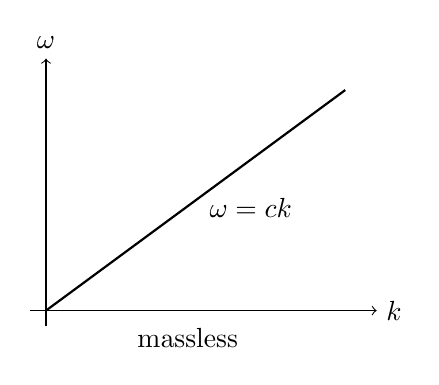
\begin{tikzpicture}[scale=1.0]
\draw[->] (-0.2,0) -- (4.2,0) node[right] {$k$};
\draw[->] (0,-0.2) -- (0,3.2) node[above] {$\omega$};
\draw[thick] (0,0) -- (3.8,2.8);
\node at (2.6,1.3) {$\omega = ck$};
\node at (1.8,-0.35) {massless};
\end{tikzpicture}
\hspace{1.2cm}
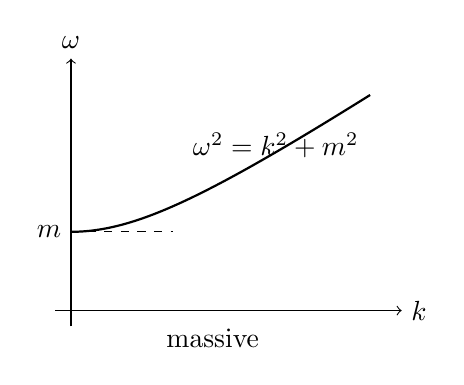
\begin{tikzpicture}[scale=1.0]
\draw[->] (-0.2,0) -- (4.2,0) node[right] {$k$};
\draw[->] (0,-0.2) -- (0,3.2) node[above] {$\omega$};
\draw[thick,domain=0:3.8,samples=100,smooth] plot (\x,{sqrt(1.0+0.45*\x*\x)});
\draw[dashed] (0,1.0) -- (1.3,1.0);
\node[left] at (0,1.0) {$m$};
\node at (2.6,2.1) {$\omega^2 = k^2 + m^2$};
\node at (1.8,-0.35) {massive};
\end{tikzpicture}
\caption{Transcript-guided redraws of the two dispersion relations that organize the opening conceptual discussion.}
\end{figure}

This is not just a particle formula. It is a statement about fields. The limit \(k=0\) means infinite wavelength, and infinite wavelength means a homogeneous displacement of the field. We shift the field everywhere in space by the same amount and let it go. If the field then oscillates with some nonzero frequency, that frequency is the mass.

This is the bridge to potential energy. Suppose we displace the field homogeneously away from equilibrium. If the potential curves upward there, the field is pulled back, overshoots, and oscillates. If the potential is flat in that direction, the field simply sits there. So the lecture turns the notion of mass into a geometric one:

\begin{itemize}
\item curvature of the potential at equilibrium means a massive mode;
\item a flat direction of the potential means a massless mode.
\end{itemize}

This is precisely the clue that makes the broken-symmetry potential useful. Once the potential has a minimum along an entire rim, motion along the rim costs no potential energy, while motion inward or outward does.

\section{Complex Scalar Field and the Broken \(U(1)\) Potential}

The next move is to introduce the field that will carry the broken symmetry. We take a complex scalar field \(\phi\). It can be written in Cartesian form,
\begin{equation}
\phi = \phi_R + i\phi_I,
\qquad
\phi^* = \phi_R - i\phi_I,
\end{equation}
or in polar form,
\begin{equation}
\phi = \rho e^{i\alpha},
\qquad
\phi^* = \rho e^{-i\alpha}.
\end{equation}
Here \(\rho\) and \(\alpha\) are not coordinates in real space. They are coordinates in \emph{field space}. At each point of real space-time the field takes a value, and that value is a point in this auxiliary complex plane.

\begin{figure}[t]
\centering

\includegraphics[width=0.62\textwidth]{lecture_08_figure_02.png}
\caption{Blackboard sketch of the complex field in polar coordinates. The board state shows the \((\phi_R,\phi_I)\) plane together with the radial variable \(\rho\) and the phase angle \(\alpha\).}
\end{figure}

\begin{figure}[t]
\centering
\begin{tikzpicture}[scale=1.3]
\draw[->] (-0.3,0) -- (3.3,0) node[right] {$\phi_R$};
\draw[->] (0,-0.3) -- (0,2.8) node[above] {$\phi_I$};
\draw[thick] (0,0) -- (2.5,1.7);
\draw (0.75,0) arc (0:34:0.75);
\node at (1.65,1.15) {$\rho$};
\node at (1.0,0.32) {$\alpha$};
\fill (2.5,1.7) circle (1.4pt);
\end{tikzpicture}
\caption{Clean redraw of the field-space picture used in the lecture.}
\end{figure}

The kinetic term may be written in either language. In Cartesian variables,
\begin{equation}
\partial_\mu\phi^*\,\partial^\mu\phi
=
\partial_\mu\phi_R\,\partial^\mu\phi_R
+
\partial_\mu\phi_I\,\partial^\mu\phi_I.
\end{equation}
So the complex field behaves as two real scalar fields. In polar variables the same term becomes
\begin{equation}
\partial_\mu\phi^*\,\partial^\mu\phi
=
\partial_\mu\rho\,\partial^\mu\rho
+
\rho^2\,\partial_\mu\alpha\,\partial^\mu\alpha.
\end{equation}
This is the form that the lecture needs, because it separates radial motion from angular motion.

A \(U(1)\)-symmetric potential is a potential that does not care about the phase. Equivalently,
\begin{equation}
V = V(\rho) = V(\phi^*\phi).
\end{equation}
The lecture does not commit to a specific polynomial form. The key point is structural: the potential depends only on \(\rho\), not on \(\alpha\). If the minimum sits at the origin, both real components are just ordinary massive fields. But if the minimum sits at some nonzero radius \(\rho=f\), then the geometry changes completely. The angular direction becomes flat.

\begin{figure}[t]
\centering

\includegraphics[width=0.8\textwidth]{lecture_08_figure_03.png}
\caption{Board layout for the radially symmetric potential discussion. The useful content is the potential sketch and the label \(V(\phi)\); the numerical examples at the far right are not part of the main argument.}
\end{figure}

\begin{figure}[t]
\centering
\begin{tikzpicture}[scale=1.0]
\draw[->] (-0.2,0) -- (4.5,0) node[right] {$\rho$};
\draw[->] (0,-0.2) -- (0,3.2) node[above] {$V(\rho)$};
\draw[thick,domain=0:4.2,samples=120,smooth]
plot (\x,{0.18*(\x-2.2)^4 - 0.95*(\x-2.2)^2 + 1.7});
\draw[dashed] (2.2,0) -- (2.2,0.35);
\node[below] at (2.2,0) {$f$};
\end{tikzpicture}
\hspace{1.2cm}
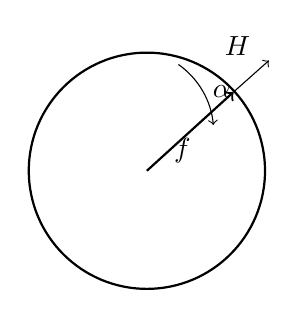
\begin{tikzpicture}[scale=1.0]
\draw[thick] (0,0) circle (1.5);
\draw[thick,->] (0,0) -- (1.1,1.0);
\draw[->] (0.4,1.35) arc (55:5:1.05);
\draw[->] (1.1,1.0) -- (1.55,1.4);
\node at (0.45,0.25) {$f$};
\node at (1.15,1.58) {$H$};
\node at (0.95,1.0) {$\alpha$};
\end{tikzpicture}
\caption{A clean reconstruction of the broken potential: a radial slice with minimum at \(\rho=f\), and a schematic rim showing the flat angular direction together with the radial Higgs fluctuation.}
\end{figure}

\subsection{Question \& Answer}

\paragraph{Question.} What is radially symmetric here: the field itself or the potential energy?

\paragraph{Answer.} The potential energy. The field at a given point in space-time is just a point in the complex plane. There is nothing radially symmetric about a single point. Radial symmetry means that the energy depends only on \(\phi^*\phi=\rho^2\), not on the angle \(\alpha\). Two field values with the same radius but different phases are assigned the same potential energy.

\section{Low-Energy Modes: Higgs and Goldstone}

Once the minimum sits at nonzero radius, it is natural to expand the radial field around the minimum:
\begin{equation}
\rho = f + H.
\end{equation}
This is the lecture's notation. The letter \(H\) is chosen because the radial fluctuation is the Higgs mode. The important physical point is that it costs a good deal of energy to push the field away from the minimum in the radial direction. The potential is steep there. By contrast, moving around the rim changes the phase but not the potential energy.

Thus the two kinds of motion have different character:

\begin{itemize}
\item radial oscillation is massive and is identified with the Higgs boson;
\item angular motion is massless and is the Goldstone boson.
\end{itemize}

At low energy we may ignore the heavy radial mode. In the language of the lecture, we freeze it. That means
\begin{equation}
\rho \approx f,
\qquad
\partial_\mu \rho \approx 0,
\qquad
V(\rho)\approx V(f).
\end{equation}
The last term is just a constant and does not affect the dynamics of the angular field. The kinetic term then reduces to
\begin{equation}
\mathcal L_{\text{low}} \approx f^2 \,\partial_\mu\alpha\,\partial^\mu\alpha.
\end{equation}
There is no mass term here. The only energy comes from spatial or temporal variation of \(\alpha\). If \(\alpha\) is shifted everywhere by the same amount, nothing happens. That is exactly what a massless mode looks like.

If we want a more familiar normalization, we simply rescale the field:
\begin{equation}
\beta = f\alpha.
\end{equation}
Then
\begin{equation}
\mathcal L_{\text{low}} \approx \partial_\mu\beta\,\partial^\mu\beta.
\end{equation}
So the Goldstone boson is a perfectly ordinary massless scalar field, but it emerged from a very special place: the flat direction of a spontaneously broken continuous symmetry.

This is where Susskind pauses and says that we have only half the story. Spontaneous symmetry breaking by itself gives us a heavy radial mode and a massless Goldstone mode. The Higgs mechanism proper requires a second ingredient: gauge invariance.

\section{From Global \(U(1)\) to Local Gauge Invariance}

After the break, the lecture deliberately backs up. This is not filler. The room is clearly struggling with what a complex field really is, so Susskind carefully distinguishes real space from the complex plane in which the field value is plotted. Only after that clarification does he review the difference between global and local phase rotations.

A global \(U(1)\) symmetry rotates the field by the same phase everywhere:
\begin{equation}
\phi(x)\to e^{i\theta}\phi(x),
\qquad
\theta=\text{constant}.
\end{equation}
This changes \(\alpha\) by a constant and leaves \(\rho\) unchanged. Since the potential depends only on \(\rho\), and since derivatives kill constants, the theory is invariant.

What fails is the corresponding local transformation
\begin{equation}
\phi'(x)=e^{i\theta(x)}\phi(x).
\end{equation}
Now the derivatives act on \(\theta(x)\) as well as on \(\phi\). Explicitly,
\begin{align}
\partial_\mu \phi'
&=
\partial_\mu\!\left(e^{i\theta(x)}\phi\right) \\
&=
e^{i\theta(x)}
\left(
\partial_\mu\phi + i(\partial_\mu\theta)\phi
\right).
\end{align}
The extra term proportional to \(\partial_\mu\theta\) is the nuisance. It is the reason the ordinary kinetic term is not invariant under local phase rotations.

\begin{figure}[t]
\centering

\includegraphics[width=0.78\textwidth]{lecture_08_figure_04.png}
\caption{Board derivation of the local phase transformation and the conclusion that the ordinary derivative term is ``not sym.''}
\end{figure}

In the lecture the conclusion is written schematically on the board as
\begin{equation}
\partial\phi^*\,\partial\phi
\neq
\partial\phi^{*\prime}\,\partial\phi'.
\end{equation}
To repair this, one introduces a compensating vector field \(A_\mu\) and replaces the ordinary derivative by the covariant derivative. The lecture's sign conventions wobble on the board, so we now choose one consistent convention and keep it fixed:
\begin{equation}
D_\mu\phi = (\partial_\mu+iA_\mu)\phi,
\qquad
D_\mu\phi^* = (\partial_\mu-iA_\mu)\phi^*,
\end{equation}
together with
\begin{equation}
A'_\mu = A_\mu - \partial_\mu\theta.
\end{equation}
Then the calculation works out cleanly:
\begin{align}
D'_\mu\phi'
&=
(\partial_\mu+iA'_\mu)e^{i\theta}\phi \\
&=
e^{i\theta}
\left(\partial_\mu+iA_\mu\right)\phi \\
&=
e^{i\theta}D_\mu\phi.
\end{align}
So the derivative of \(\theta\) has disappeared from the transformed covariant derivative. Only an overall phase remains, and that cancels against the conjugate one when we form
\begin{equation}
D_\mu\phi^*\,D^\mu\phi.
\end{equation}

The gauge field also has its own invariant curvature,
\begin{equation}
F_{\mu\nu}=\partial_\mu A_\nu-\partial_\nu A_\mu.
\end{equation}
Under the same gauge transformation,
\begin{align}
F'_{\mu\nu}
&=
\partial_\mu A'_\nu-\partial_\nu A'_\mu \\
&=
F_{\mu\nu}
-\partial_\mu\partial_\nu\theta
+\partial_\nu\partial_\mu\theta \\
&=
F_{\mu\nu},
\end{align}
because mixed partial derivatives commute.

At the board this is summarized schematically by the gauge-invariant toy Lagrangian
\begin{equation}
\mathcal L_{\text{toy}}
=
D\phi^*\,D\phi - V(\phi^*\phi) + F^2.
\end{equation}
This is lecture shorthand. In more explicit notation one may read the same statement as
\begin{equation}
\mathcal L_{\text{toy}}
=
D_\mu\phi^*\,D^\mu\phi
-
V(\phi^*\phi)
+
F_{\mu\nu}F^{\mu\nu},
\end{equation}
with the understanding that overall signs and normalizations of the Maxwell term depend on convention and were kept schematic in the lecture itself.

\begin{figure}[t]
\centering

\includegraphics[width=0.78\textwidth]{lecture_08_figure_05.png}
\caption{Secondary board summary: the schematic gauge-invariant scalar-gauge Lagrangian appears together with the remembered expansion \(\rho=f+H\).}
\end{figure}

\subsection{Question \& Answer}

\paragraph{Question.} Why is the local phase rotation not already a symmetry of the scalar kinetic term?

\paragraph{Answer.} Because \(\partial_\mu\) differentiates everything that depends on \(x\). If the phase is constant, the derivative never sees it. If the phase is \(\theta(x)\), the derivative produces the extra term \(i(\partial_\mu\theta)\phi\). The ordinary derivative therefore transforms badly. The covariant derivative is invented precisely to cancel that term.

\section{The Higgs Mechanism in the Toy Gauge Theory}

We now put the two halves together. The broken scalar theory gave us a heavy radial mode and a massless angular mode. The gauge theory gave us a massless vector field with a covariant derivative. What happens when both structures are present at once?

First, why is the photon massless in the unbroken gauge theory? Because its energy is built from \(F_{\mu\nu}\), and \(F_{\mu\nu}\) contains only derivatives of \(A_\mu\). If we shift \(A_\mu\) homogeneously everywhere, there is no change in \(F_{\mu\nu}\), hence no change in energy. That is the same \(k=0\) logic from the beginning of the lecture.

If one tried to write a direct mass term, it would look like
\begin{equation}
A_\mu A^\mu.
\end{equation}
But this is not gauge invariant:
\begin{equation}
A_\mu A^\mu
\;\longrightarrow\;
(A_\mu-\partial_\mu\theta)(A^\mu-\partial^\mu\theta),
\end{equation}
which is not the same expression. So gauge invariance forbids the obvious mass term.

Now comes the real point. Near the broken minimum, and at low energy, we may freeze the radial mode and write
\begin{equation}
\phi(x)\approx f e^{i\alpha(x)}.
\end{equation}
Insert this into the covariant derivative:
\begin{align}
D_\mu\phi
&\approx
(\partial_\mu+iA_\mu)\bigl(f e^{i\alpha}\bigr) \\
&=
i f e^{i\alpha}\bigl(\partial_\mu\alpha + A_\mu\bigr).
\end{align}
Therefore
\begin{equation}
|D_\mu\phi|^2
\approx
f^2\bigl(\partial_\mu\alpha + A_\mu\bigr)
\bigl(\partial^\mu\alpha + A^\mu\bigr).
\end{equation}
This is the combination the lecture is trying to isolate in the final derivation. Up to conventional factors, it is exactly the structure one needs.

Now choose the gauge transformation
\begin{equation}
\theta(x)=-\alpha(x).
\end{equation}
Then
\begin{equation}
\phi'(x)=e^{i\theta(x)}\phi(x)=f,
\qquad
A'_\mu = A_\mu + \partial_\mu\alpha.
\end{equation}
So the angular field disappears from the scalar altogether, and the covariant-derivative term becomes
\begin{equation}
|D_\mu\phi|^2 \to f^2 A'_\mu A^{\mu\prime}.
\end{equation}
In other words, the theory has generated an effective mass term for the gauge field out of a perfectly gauge-invariant expression. This is the Higgs mechanism in its simplest abelian form.

There is a useful conceptual point here. We did \emph{not} add the forbidden term \(A_\mu A^\mu\) by hand. We got it from the covariant derivative after the scalar field settled at nonzero magnitude. That is why gauge invariance is not really violated. It is realized in a more subtle way.

The lecture then immediately returns to the superconductor. The charged boson field there is the condensate of Cooper pairs. Once that charged condensate forms, the electromagnetic field inside the material behaves just as this toy theory predicts: the photon acquires an effective mass.

\subsection{Question \& Answer}

\paragraph{Question.} Where did the Goldstone boson go, and how can no degree of freedom be lost?

\paragraph{Answer.} The Goldstone mode was the phase field \(\alpha(x)\). But in a gauge theory a space-time dependent phase can be absorbed into a gauge transformation. So the would-be Goldstone boson is not an independent physical excitation once the symmetry is gauged. Its degree of freedom reappears as the longitudinal polarization of the now-massive vector boson.

This is exactly the degree-of-freedom bookkeeping emphasized in the lecture:
\begin{equation}
2\ \text{(massless photon polarizations)}
+
2\ \text{(real scalar components)}
\;\longrightarrow\;
3\ \text{(massive vector polarizations)}
+
1\ \text{(Higgs scalar)}.
\end{equation}
A massless photon has only two transverse polarizations because it can never be brought to rest. A massive vector boson can be brought to rest, so it must have three polarizations. The missing third one is precisely what the would-be Goldstone mode supplies.

\section{Summary}

The lecture proceeds in a very deliberate order, and the logic is now visible. We began by distinguishing a genuine mass from a mere change in propagation speed. Mass is the frequency of the homogeneous mode at \(k=0\), and in field language it comes from curvature of the potential. A broken \(U(1)\)-symmetric scalar potential therefore produces two kinds of motion: a heavy radial Higgs mode and a massless angular Goldstone mode.

Gauge invariance supplies the second half. A local phase rotation is not a symmetry of the ordinary kinetic term, so we introduce the vector potential \(A_\mu\), the covariant derivative, and the field strength \(F_{\mu\nu}\). Once the scalar field sits at nonzero magnitude, the covariant derivative produces the combination \(\partial_\mu\alpha + A_\mu\). A gauge choice removes \(\alpha\), and what remains is a mass term for the gauge field. The Goldstone boson has not been destroyed; it has become the longitudinal polarization of the massive vector boson. That is the abelian Higgs mechanism, and it is the toy model for how gauge bosons acquire mass in the Standard Model.